\chapter{Tools}

\section{Monitoring}

In the monitoring phase the user is supposed to collect log files
relative to correct system executions. These log files can be
collected at testing time during functional system tests or during
correct runs of the system. We do not provide any logging tool
because the system can work with any logging systems.

\section{Model Generation}

In this phase the log files collected are analyzed by the system to
derive a model that generalizes the application behavior.
In this phase the initial logs files are preprocessed with different
tools in order to:
\begin{itemize}
 \item contain a complete event in a single line;
\item automatically detect event types and associated parameters;
\item detect rewriting strategies for parameters;
\item infer a model of the log file structure;
\end{itemize}

Figure \ref{fig:modelGenerationComponents} shows the components
involved
in this phase. All the components must be called from command line
and the user has to set parameters according to the analysis type and
the log file analyzed. Following sections describe the functionality
of each component. 

\begin{figure*}[ht!]
    \begin{center}
        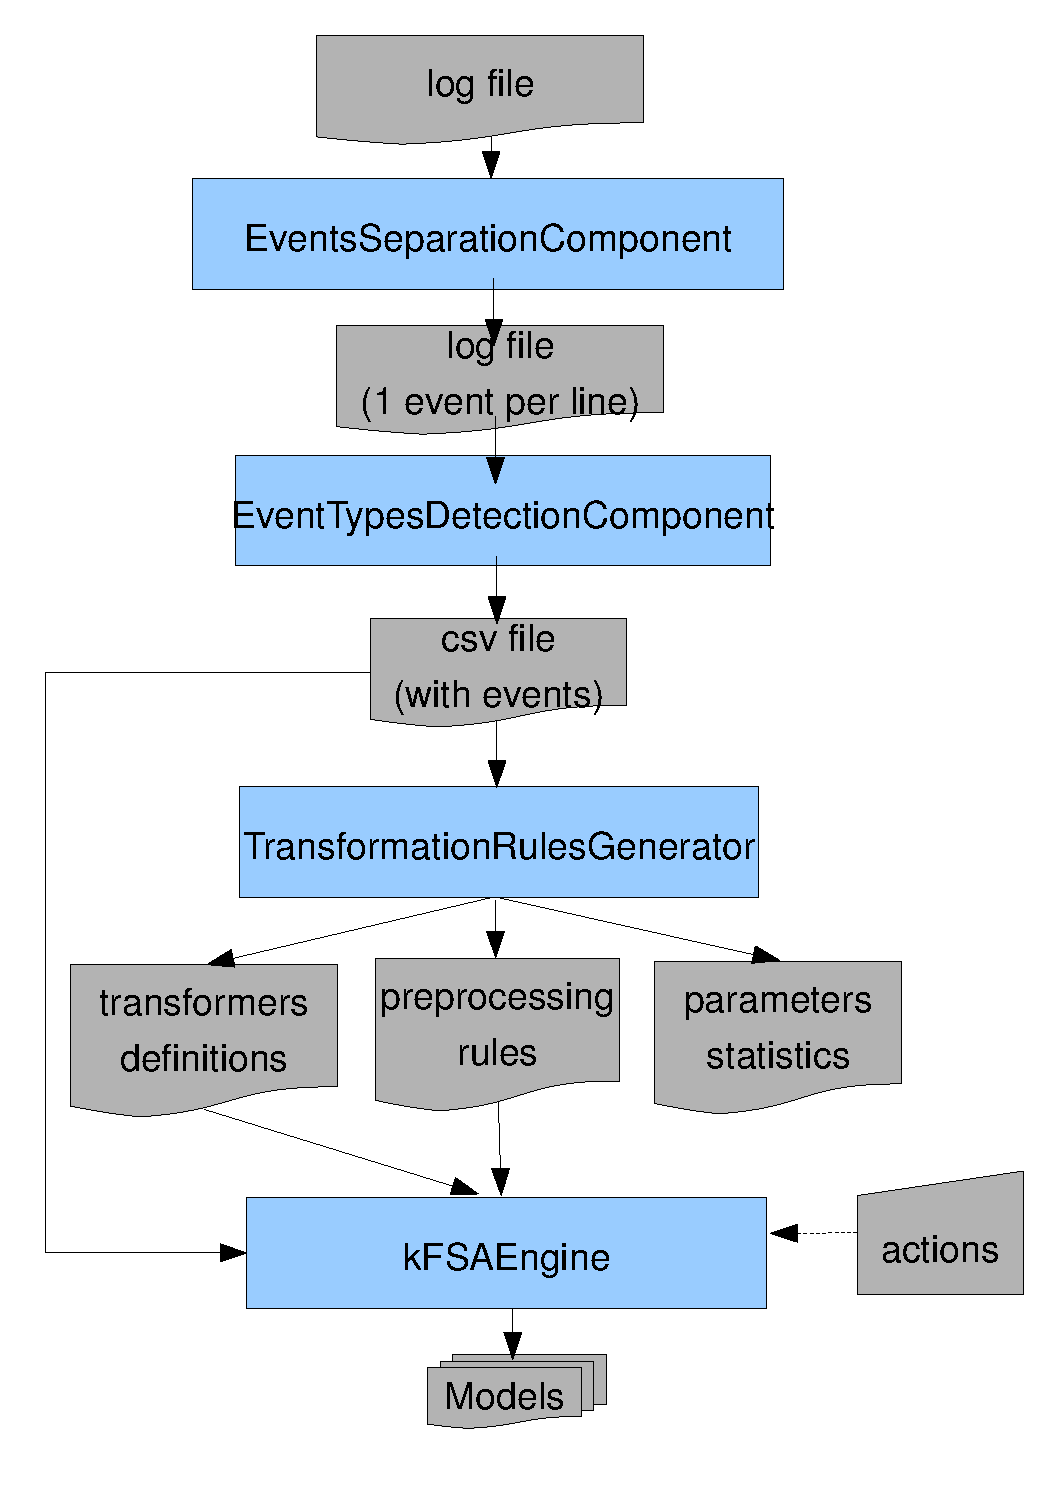
\includegraphics[width=12cm]{images/modelGeneration}
    \end{center}
    \caption{Components involved in the model generation phase.}
\label{fig:modelGenerationComponents}
\end{figure*}

\section{Failure Analysis}

In this fail the logs recorded during faulty executions are first
preprocessed following the criterion adopted in the model inference
phase and then are compared with the inferred models.

Figure~\ref{fig:failureAnalysis} shows the components involved in this
phase.


\begin{figure*}[ht!]
    \begin{center}
        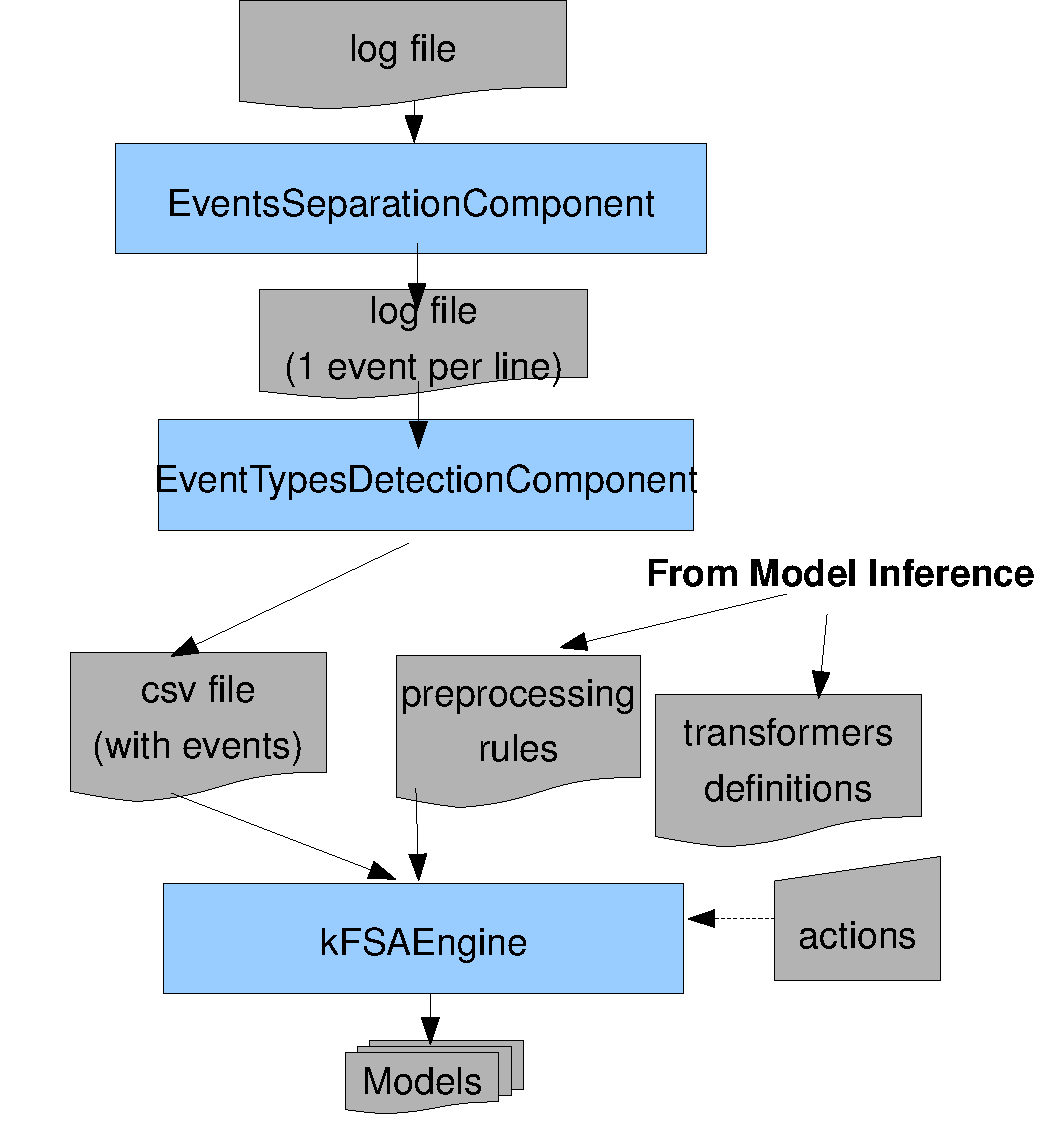
\includegraphics[width=12cm]{images/failureAnalysis}
    \end{center}
    \caption{Components involved in the failure analysis phase.}
\label{fig:failureAnalysis}
\end{figure*}


The results of this phase are a set of extended models and an anomaly file. 
%The anomaly file contains the colums described in Table~


\begin{table}
% \title{Preliminary description of C}
\begin{tabular}{|p{6cm}|p{10cm}|}
\hline
Column name&Description\\
\hline
Component&Name of the component that presents this anomaly.\\
Anomaly&Anomaly type, can be branch, tail or final state.\\
Line&Position in the trace in which the anomaly starts. 
This number corresponds to the position of the event in the trace named
checking\_<componentName>.trace \\ 
State&State of the component FSA in which the anoamly has been found\\
StateType& State type, can be \textit{existing} if it is a state present in the 
component FSA, or \textit{new}if it is a state added during a previous extension\\
Event&Sequence of anomalous preprocessed events observed\\
Original log line&Position in the original log\\
Original log event&Sequence of anomalous events observed\\
To state&State in which the anomaly ends (makes sense only if it is a branch
added anomaly). \\
Branch length&Lenght of the added branch.\\
Expected&Expected event going out from the anomalous state\\
Expected incoming&Events expected before state "To state"\\
\hline 
\end{tabular}
\end{table}  
